% REMEMBER: You must not plagiarise anything in your report. Be extremely careful.

\documentclass{l4proj}
\graphicspath{ {./images/} }
    
%
% put any additional packages here
%

\begin{document}

%==============================================================================
%% METADATA
\title{Multilingual News Collection and Classification}
\author{Adam Fairlie}
\date{January 30, 2023}

\maketitle

%==============================================================================
%% ABSTRACT
\begin{abstract}
    Every abstract follows a similar pattern. Motivate; set aims; describe work; explain results.
    \vskip 0.5em
    ``XYZ is bad. This project investigated ABC to determine if it was better. 
    ABC used XXX and YYY to implement ZZZ. This is particularly interesting as XXX and YYY have
    never been used together. It was found that  
    ABC was 20\% better than XYZ, though it caused rabies in half of subjects.''
\end{abstract}

%==============================================================================

% EDUCATION REUSE CONSENT FORM
% If you consent to your project being shown to future students for educational purposes
% then insert your name and the date below to  sign the education use form that appears in the front of the document. 
% You must explicitly give consent if you wish to do so.
% If you sign, your project may be included in the Hall of Fame if it scores particularly highly.
%
% Please note that you are under no obligation to sign 
% this declaration, but doing so would help future students.
%
%\def\consentname {My Name} % your full name
%\def\consentdate {20 March 2018} % the date you agree
%
\educationalconsent


%==============================================================================
\tableofcontents

%==============================================================================
%% Notes on formatting
%==============================================================================
% The first page, abstract and table of contents are numbered using Roman numerals and are not
% included in the page count. 
%
% From now on pages are numbered
% using Arabic numerals. Therefore, immediately after the first call to \chapter we need the call
% \pagenumbering{arabic} and this should be called once only in the document. 
%
% Do not alter the bibliography style.
%
% The first Chapter should then be on page 1. You are allowed 40 pages for a 40 credit project and 30 pages for a 
% 20 credit report. This includes everything numbered in Arabic numerals (excluding front matter) up
% to but excluding the appendices and bibliography.
%
% You must not alter text size (it is currently 10pt) or alter margins or spacing.
%
%
%==================================================================================================================================
%
% IMPORTANT
% The chapter headings here are **suggestions**. You don't have to follow this model if
% it doesn't fit your project. Every project should have an introduction and conclusion,
% however. 
%
%==================================================================================================================================
\chapter{Introduction}

% reset page numbering. Don't remove this!
\pagenumbering{arabic} 


Why should the reader care about what are you doing and what are you actually doing?
\section{Motivations and Aims}

\textbf{Motivate} first, then state the general problem clearly. 

\section{Chapter outline}

%==================================================================================================================================
\chapter{Background and Research}
What did other people do, and how is it relevant to what you want to do?
\section{Digital News Surveillance Systems}
\subsection*{BioCaster}
This project reworks and extends some of the digital news surveillance system currently used in \cite{biocaster}. The system collects news articles through a variety of RSS,  feeds using a Perl script, across different languages including English, French and Mandarin Chinese \citep{collier2008biocaster}. It uses a machine translation server to translate the headlines and descriptions into English, and a machine learning model built on PubMedBERT \citep{gu2021domain} to classify whether news articles are related to disease outbreaks \citep{meng2022biocaster}. It also uses text mining approaches with BioSyn \citep{sung2020biomedical} to perform entity extraction and linking, in order to determine details of the disease outbreak such as the disease type and who it is currently affecting. It also uses Early Aberration and Reporting System (EARS) algorithms, will classify the risk level of the outbreak \citep{collier2011towards}. 
\begin{figure}[h]
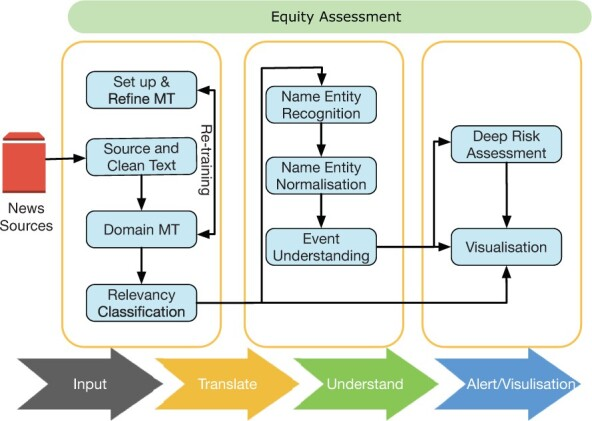
\includegraphics[width=\textwidth]{/biocaster_diagram.jpg}
\caption{The full architecture of the current BioCaster app. Image obtained from \cite{meng2022biocaster}}
\label{fig:biocaster_architecture}
\end{figure}
\par
The later stages of this process are outside the scope of this project. The current BioCaster data collection system is dated, relying on PERL and only collecting data through RSS feeds, which are only provided by some (typically larger, more common language) news sources. This greatly limits the amount of data which can be extracted, particularly from smaller sources in minority languages, which are underrepresented in disease tracking systems (citation needed). This project will develop a more modern system for collecting the RSS data in Python, as well as functionality for using web scraping to collect news articles from webpage HTML. The system will be designed so that it is easily extensible to other sources of data which may be more prominent in different countries, such as social media posts. This also allows for entire article text to be collected instead of just the headline and a short description, which may allow for a richer understanding of the news content and more effective performance in ML tasks.

\subsection*{Other BioMedical Systems}
HealthMap, GPHIN, ProMED Mail, MedISys, Argus, EpiSPIDE, EpiCore.
Web crawler with keyword filtering \citep{zhang2009automatic}
\subsection*{Other Systems}
Meltwater, Cision, Muck Rack, Agility PR Solutions (Marketing, brand management/PR etc.).


\section{Web Scraping Technologies}
The main free and open-source technologies for scraping news articles from websites in Python were Newspaper3K and news-please, which is built on top of Newspaper3K and adds some extra features \citep{newspaper3k, news-please}. Another option considered was Newscatcher \citep{newscatcher}, but the free API is limited in how many calls can be made and this made it unsuitable for this project. Finally, I looked at pygooglenews \citep{pygooglenews} which provided some promise in using google news to find articles under certain subjects, keywords, languages and regions. For this project, I found it desirable to have better control of the exact sources collected, instead of filtering through keywords and relying on Google's source selection, but a scraper using this library could easily be added to extend the capabilities of the current system. I decided to move forward with the former two libraries and conducted an experiment to compare their capabilities. \par

I compared the features present in each of the two libraries. Notably, Newspaper3K can perform full website scraping in Python, whereas news-please can only do this using its Command Line Interface (CLI). I attempted to scrape 3 articles from each of the 109 previously selected websites, across 10 languages, and compared the number of successful scrapes (without error) and the average speed. The results are shown below: \par 
(Results table) \par
Newspaper3K scraped 103 of the 109 websites (94.5\%) without error, whereas news-please scraped 102/109 (93.58\%). The average scraping times are similar in both libraries, but Newspaper3K was faster at scraping in 8 of the 10 languages, and average scraping time per article was 14.82\% lower, Based on these factors, I chose to use Newspaper3K for the scraping system.

\section{Database and Visualisation}
The visualisation was mainly inspired by the current \cite{biocaster} interface, available on their website. This design had to be updated to reflect the changes from my project to the current system, including the addition of news article topics and different source types of information retrieved. I also did not have the specific region or disease information to create the alerts seen on the BioCaster interface. In addition, I chose to change the article density to cover the whole country, to make the source of the data more visible (so that it does not obstruct the view of other countries) and created a monochromatic green colour map, where darker colours represented more articles retrieved as is common practice in world density maps \citep{ourworldindata_density, ons_density}.
\begin{figure}[h]
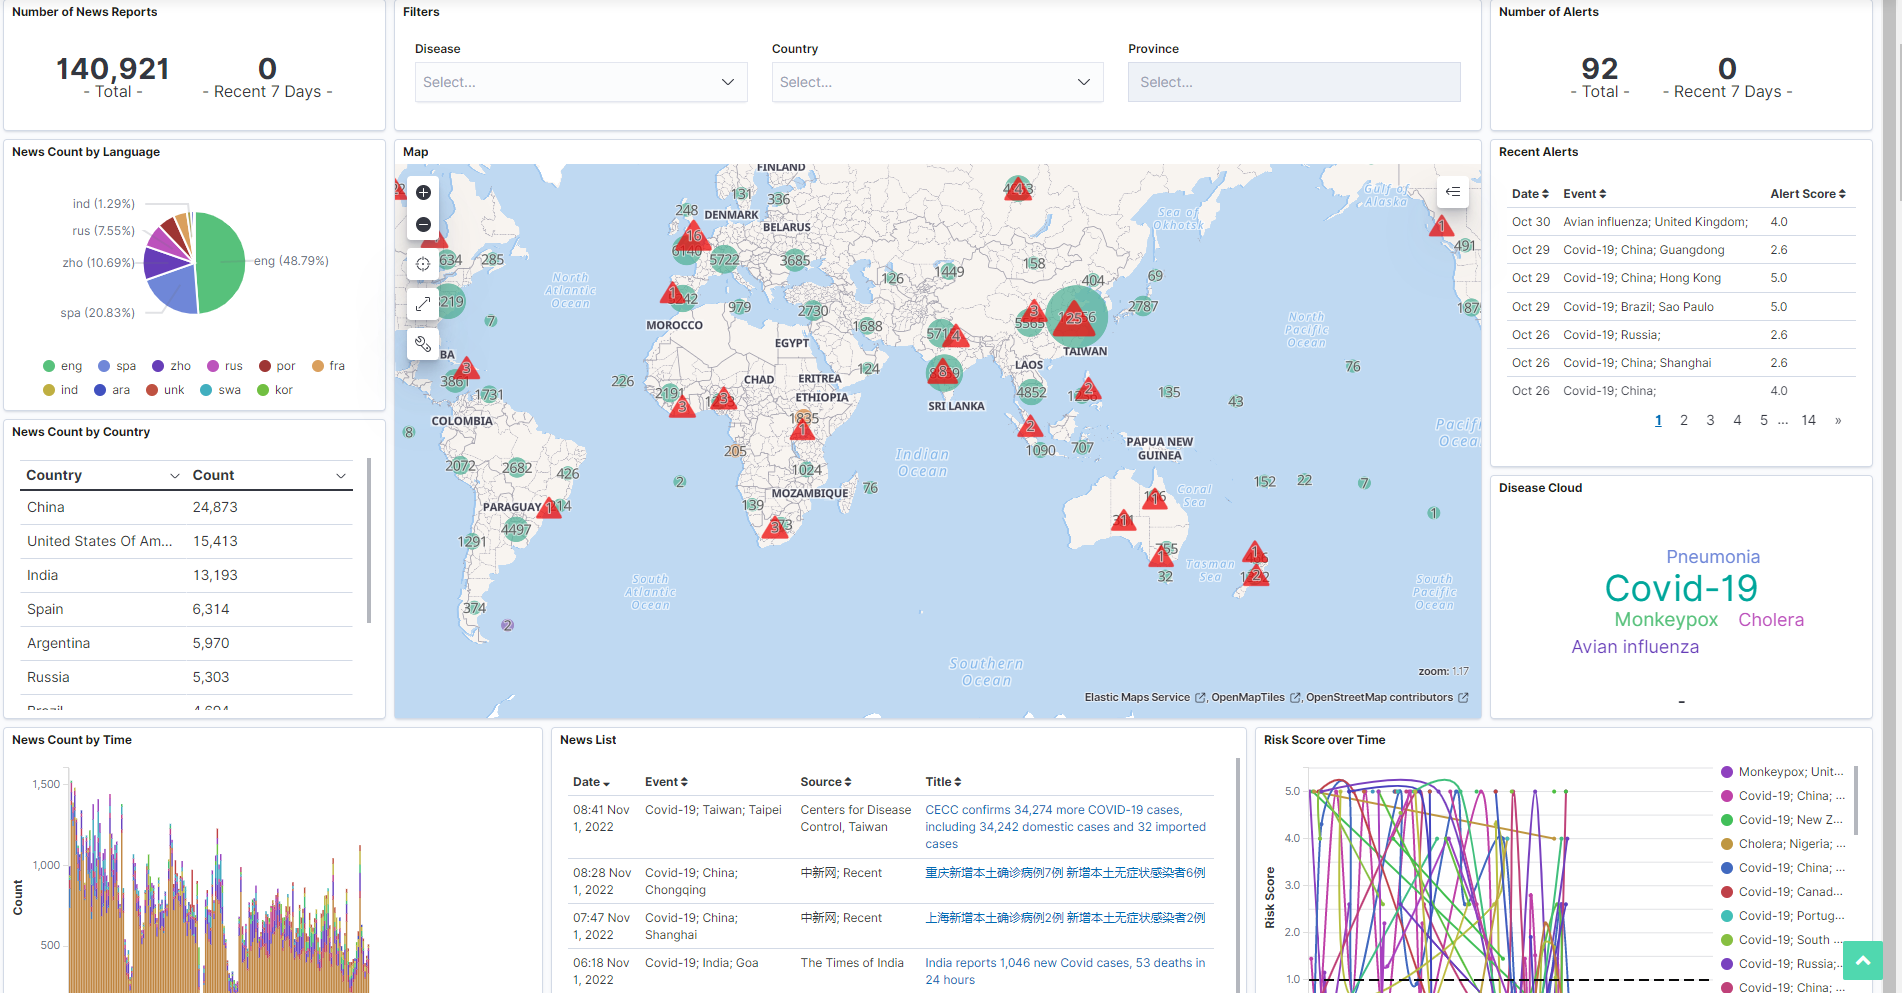
\includegraphics[width=\textwidth]{/biocaster_interface.png}
\caption{BioCaster Kibana Visualisation (from the homepage)}
\label{fig:biocaster_visualisation}
\end{figure}
\par
The BioCaster visualisations are created using the Elastic stack, storing the data with elasticsearch and creating visualisations using Elastic Kibana \citep{elastic_stack}. After originally using MySQL with the Python MySQL connector to store the data from the scraping system, and considering standard python visualisation libraries such as matplotlib \citep{Hunter:2007} and geoplotlib \citep{geoplotlib} for geographical data, I decided to also use the Elastic stack, using the elasticsearch Python library to integrate the scraping system into the database.

\section{News Article Classification}
\subsection{Datasets}
\subsection{Models}
\section{Web Interface}
\section{Ethical / Legal Considerations}


%==================================================================================================================================
\chapter{Requirements}
\section{Functional Requirements}
\section{Non-functional Requirements}

%==================================================================================================================================
\chapter{Implementation}
\section{Design Choices}
\subsection{Web Scraping Technology}
\subsection{Classifier Model}
\subsection{Visualisation}
\subsection{Web Interface}
\section{Web Scraping System}
\section{Database}
\section{Visualisations}

\section{News Article Classification}
\subsection{Research Questions}
The research question I aim to answer is \emph{"Are multilingual models effective for multilingual multi-topic news classification?"} and \emph{"What is the most effective model in this setting?"}
\subsection{Data Collection}
Data will be collected through the scraping system previously developed, using articles which have been labelled by the source as one of 6 categories: Health, Sports, Entertainment, Business/Finance, Politics and Technology. For some sources, categories with similar names (e.g. "Wellness" and "Health") have been merged. A full list of sources and category keywords used can be found in the appendices.
\subsection{Model and Parameter Choices}
Previous research for monolingual research has shown that Multinomial Naive Bayes models have been effective in multi-topic news classification. I will optimise the alpha (smoothing) parameter through a randomised grid search. I will compare this model to a fine-tuned uncased BERT model. For multilingual classification, I will compare 2 fine-tuned BERT-based models: Multilingual uncased BERT and XML-RoBERTa.
\subsection{Data Transformations}
In the case of the monolingual models, sentences will be translated into English before classification. As is common in article classification research, the article headline and body will be concatenated into one column. In the Naive Bayes model, words will be tokenised and stemmed, and tokens will be converted into TF-IDF feature vectors. In the deep learning models (Monolingual/multilingual bert, XML-RoBERTa) The text will be converted into word embeddings by the BERT tokeniser. In all cases, data will be truncated to 256 tokens, and padded if necessary.
\subsection{Evaluation}
The performance of each model will be evaluated on its accuracy and micro-f1 score. Confusion matrices for each model type will also be shown in the appendices. I will use a most frequent dummy classifier as a baseline for model effectiveness.

\section{Web Interface}
%==================================================================================================================================
\chapter{Evaluation}
\section{Automatic Web Scraping System}
\section{News Article Classification}
\section{Web Interface and Visualisations}
\subsection{Accessibility}
\subsection{Usability Testing}
\section{Project Limitations} 

%==================================================================================================================================
\chapter{Conclusion}    
Summarise the whole project for a lazy reader who didn't read the rest (e.g. a prize-awarding committee).
\section{Project Summary}
\section{Future Work}
%==================================================================================================================================
%  APPENDICES  
\begin{appendices}

\end{appendices}

%==================================================================================================================================
%   BIBLIOGRAPHY   
\bibliographystyle{abbrvnat}
\bibliography{l4proj}

\end{document}
